\documentclass[10pt,twocolumn,letterpaper]{article}
\usepackage[review]{cvpr}
\usepackage{amsmath,amssymb,booktabs,multirow,graphicx}
\usepackage[pagebackref,breaklinks,colorlinks]{hyperref}
\def\confName{CVPR}
\def\confYear{2027}
\setlength{\tabcolsep}{3pt}
\newcommand{\R}{\mathbb{R}}
\newcommand{\spn}{\operatorname{softplus}}
\newcommand{\tr}{\operatorname{tr}}
\newcommand{\dev}{\operatorname{dev}}
\newcommand{\diag}{\operatorname{diag}}
\newcommand{\file}[1]{\texttt{\small\detokenize{#1}}}
\title{Compositional Neural Mechanics for Physical Prediction Beyond Visual Agreement\\Supplementary Material}
\author{Anonymous submission}
\begin{document}
\maketitle
\section{Scope and experimental map}
This supplement specifies the implemented models, numerical methods, experimental accounting, and limitations. The preceding evidence comprises three distinct settings: (i) static composition with oracle physical descriptors, (ii) static inference of 15 continuous unknown descriptors and acquisition of an additional position observation, and (iii) dynamic calibration followed by larger-drop prediction against a native PhysTwin adaptation. A fourth study extends dynamic prediction to six coupled-scene families with unknown materials and known boundaries; its protocol is specified in Sec.~\ref{sec:complex-scenes-supp}. Results from these settings are not interchangeable. In particular, the dynamic experiment does not evaluate the static active policy or its uncertainty model.

The central representation is a reusable, conditional \emph{energy law}. A small shared network maps physical descriptors to coefficients of invariant energy functions. A conventional mechanics solver combines this bulk law with attachment and contact potentials. Scene-specific inference estimates descriptors while the shared network weights remain frozen. Gaussian appearance is attached to material coordinates and transported by the resulting deformation. The system does not learn a direct image-to-force map, reconstruct unknown topology, or learn friction from video.

\paragraph{Units and metric conventions.}
Coordinates and tool translations are in metres; rotation vectors are in radians; force is in newtons; torque is in newton-metres. Bulk energy density is in pascals, total energy in joules, attachment stiffness in N/m, and normal-contact stiffness density in N/m$^3$. Static tables report \emph{coordinate} RMSE. Dynamic benchmark tables report \emph{point-vector} RMS, which is $\sqrt{3}$ times coordinate RMS for identical samples and weights. Numerical qualification thresholds remain in their originally declared coordinate convention.

\paragraph{What is shared.}
The bulk and bilateral-interface networks are frozen across objects and mechanical compositions. Reference geometry, material-coordinate fields, prescribed tool poses, gravity, and collision geometry enter the solver explicitly. Gravity is an external body load, rather than an output of the interface network. The dynamic drop study uses the shared bulk law and analytic normal contact; bilateral learned interfaces are evaluated in the static composition study, not covertly inserted into a free-body drop.

\paragraph{What is conventional.}
Invariant hyperelasticity, finite elements, sparse Newton solves, penalty contact, consistent mass, Verlet integration, implicit differentiation, and affine covariance transport are established ingredients. Our implementation combines them with shared conditional laws and auditable descriptor inference. We do not claim a new finite-element formulation, proof of polyconvexity, a general collision engine, or calibrated uncertainty.

\begin{figure}[t]
\centering
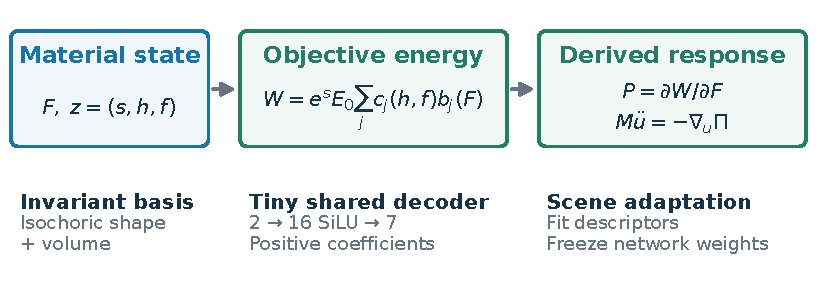
\includegraphics[width=\linewidth]{figures/energy_block.pdf}
\caption{Shared conditional energy components are composed by the mechanics solver. Frozen constitutive weights are distinct from inferred scene descriptors and from transported appearance.}
\label{fig:energy-supp}
\end{figure}
\section{Conditional bulk energy}
Let $X$ be a material coordinate, $x(X)=X+u(X)$ the deformation, $F=\partial x/\partial X$, $J=\det F>0$, and $C=F^\top F$. Define
\begin{align}
 I_1&=\tr C, & I_2&=\tfrac12[(\tr C)^2-\tr(C^2)],\\
 q_1&=J^{-2/3}I_1-3, &q_2&=J^{-4/3}I_2-3,\\
 v(J)&=J-\log J-1.
\end{align}
The shared bulk energy is
\begin{equation}
 W_\theta(F;s,h,c)=e^s E_0\,a_\theta(h,c)^\top b(F),\qquad E_0=12000\ \mathrm{Pa},
\end{equation}
with
\begin{equation}
 b=[q_1/2,q_2/2,v,q_1^2,q_1^3,\phi_1(q_1),\phi_2(q_1)]^\top,
\end{equation}
\begin{align}
 a_\theta&=\spn(\mathrm{MLP}_\theta(h,c))+10^{-8},\\
 \phi_i(q)&=\spn(\alpha_iq)-\log2-\alpha_iq/2,\\
 \alpha_i&=\spn(\rho_i)+10^{-4}.
\end{align}
The coefficient decoder has two inputs, one 16-unit SiLU hidden layer, and seven outputs. Including the two slopes, it contains 169 parameters. The descriptor $s$ is a log common stiffness scale; $h$ controls nonlinear material shape; $c=-1$ and $+1$ designate the two teacher families. The scale enters only as $e^s$, not through the decoder. Spatial heterogeneity is represented through a material-coordinate descriptor field, rather than a separate network per object.

Objectivity and isotropy follow from the invariants. The reference energy and stress vanish at $F=I$. Stress $P=\partial W/\partial F$ and tangent $\partial P/\partial F$ are evaluated by automatic differentiation. Positive coefficients and reference normalization do not imply global convexity in $F$, uniqueness of equilibrium, or unconditional stability. The implementation rejects nonpositive determinants and applies additional sampled determinant guards during solves.

\section{Constitutive pretraining and interface laws}
\subsection{Bulk teachers and training}
The two analytic teacher families share small-strain moduli but differ at finite strain. With $a=\operatorname{sigmoid}(h)$, $\mu=4000e^s$ Pa, $K=20000e^s$ Pa, and $f=.15+.6a$,
\begin{align}
 W_{\rm MR}&=\frac{\mu}{2}[(1-f)q_1+fq_2]+Kv,\\
 W_{\rm Y}&=\mu\left[\tfrac12q_1+(.08+.3a)q_1^2\right.\nonumber\\
 &\hspace{32mm}\left.+(.01+.08a)q_1^3\right]+Kv.
\end{align}
These laws should not be confused with the separate stable-Neo-Hookean engine-control experiments.

Bulk pretraining uses 18 descriptor combinations: three scales $s\in\{-.5,0,.5\}$, three shapes $h\in\{-1,0,1\}$, and both families. There are 4096 training strain coupons and 512 validation coupons. Deformation gradients are upper triangular with log diagonal entries sampled in $[-.2,.2]$ and upper off-diagonal entries in $[-.4,.4]$. This supplies positive determinants. The objective is
\begin{equation}
\begin{aligned}
 \mathcal L_W={}&\operatorname{MSE}(P_\theta/12000,P_*/12000)\\
 &+.1\operatorname{MSE}(W_\theta/12000,W_*/12000).
\end{aligned}
\end{equation}
Training uses float64, batch size 256, 6000 fixed Adam steps, initial learning rate $.003$, and cosine decay. The final iterate is frozen before generating constitutive test coupons. No scene trajectories, reserved-object targets, or rendered future images are used to train this law. The tested interpolation descriptors use scales $\pm.25$ and shapes $\pm.5$; a harder strain test extends the log-diagonal/shear ranges to $.35/.7$.

\subsection{Compliant bilateral attachments}
For a tool with reference origin $c_b$, translation $t_b$, and rotation $R_b$, define
\begin{equation}
 \delta_b(X)=x(X)-\{c_b+t_b+R_b(X-c_b)\}.
\end{equation}
The attachment is a bilateral compliant potential, not a unilateral collision constraint. Let $r=\|\delta\|^2/\ell^2$, with $\ell=.002$m. Its learned law is
\begin{equation}
 \psi_\theta(\delta;K,\chi,f)=\tfrac12K\ell^2\left[r+2\chi\sum_{j=1}^{7}a_j(\chi,f)\phi_j(r)\right].
\end{equation}
The bases comprise $r^2$ and six functions
\begin{equation}
 \phi_j(r)=\spn(b_j+\alpha_jr)-\spn(b_j)-\sigma(b_j)\alpha_jr.
\end{equation}
A two-input, 16-unit Tanh, seven-output decoder produces positive coefficients; six slopes and six offsets are also learned. There are 179 parameters. The outer stiffness factor is $K$, in N/m. At $\chi=0$ the interface is exactly quadratic. Tractions and tangents are derivatives of this scalar potential.

The analytic interface teachers use
\begin{equation}
 \psi_* =\tfrac12K\ell^2\{r+2\chi[(1-f)r^2+f(r-\log(1+r))]\},
\end{equation}
where $f=0$ is polynomial and $f=1$ is saturating in its nonlinear correction. The final wide-range checkpoint warm-starts the earlier small-slip model. Its 16384 coupons comprise equal numbers with radii up to $3\ell$ and $16\ell$, and strengths $.1,.3,.5,.7,.9$. Training uses 6000 fixed Adam steps, batch 512, initial learning rate $.003$, final rate $.0003$, and gradient clipping at 1. Force and energy residuals are normalized by $K\ell+\|t_*\|$ and $K\ell^2+|\psi_*|$, respectively, with energy weight $.05$. A failed wide-range random initialization remains recorded; it is not substituted into the final method.

\subsection{Spatial interface fields}
Attachment weights are reference-area weights multiplied by a Gaussian footprint and a smooth boundary taper, then normalized to sum to one. On normalized face coordinates $q=(q_y,q_z)$, the footprint is proportional to
\begin{equation}
 \prod_{d=y,z}4q_d(1-q_d)\exp\left[-\tfrac12\sum_{d=y,z}\left(\frac{q_d-c_d}{w_d}\right)^2\right].
\end{equation}
Centers $c_d$ and log-widths $\log w_d$ can be unknown continuous descriptors. Normalization makes $K$ a total attachment stiffness rather than a mesh-dependent per-node constant. The weights are differentiable with respect to the centers and widths. Reactions and torques use the same integrated potential and current contact/attachment locations.

\paragraph{Scale ambiguity.}
For zero independent body load and fixed prescribed tool poses, multiplying all bulk and interface stiffnesses by $\alpha>0$ gives $\Pi_\alpha(u)=\alpha\Pi(u)$. Consequently the stationary and minimizing sets are unchanged, while reaction forces and tangents scale by $\alpha$. Position-only data cannot determine this common scale. This is a statement about a specified load model, not global identifiability. Known gravity or known-mass timed dynamics can break the symmetry. A contact term must also be co-scaled for this identity; fixed numerical contact compliance otherwise provides a relative scale.

\section{Forward solver, contact and motion}
\subsection{Finite-element discretization}
The displacement field is interpolated with tensor-product quadratic hexahedral basis functions. Each element has 27 nodes, and the structured layout is $(4n,n,n)$ elements. Thus $n=2,3,4,6,8$ correspond to 425,1225,2673,8281,18785 nodes, respectively. The parameter $n$ is not the total number of elements per direction. Geometry maps support variations of length, width, depth, taper and arch; arbitrary topology is not inferred.

The discrete potential is
\begin{equation}
 \Pi(u)=\sum_q w_q W_\theta(F_q,z_q)+\sum_b\sum_{q\in b}\bar w_q\psi_\theta(\delta_q,z_b)+\Pi_c(u)-f_g^\top u.
\end{equation}
Reference-volume and reference-area quadrature are explicit. Static equilibria use sparse Newton iterations with a checked linear residual, descent check and Armijo backtracking. Tangents are energy derivatives. Determinants are checked at quadrature locations and element check points, including nodal locations; these sampled checks are not a global continuous-element positivity certificate. Continuation within a prescribed action improves equilibrium initialization without treating a sequence of unrelated probes as a physical dynamic trajectory.

\subsection{Unilateral normal contact}
For a known plane or sphere signed distance $g(x)$,
\begin{equation}
 \Pi_c=\frac12 k_c\int_{\Gamma_0}\min(g(x),0)^2\,dA_0.
\end{equation}
The surface points follow the current Q2 deformation, while the integration measure is reference area. The stiffness $k_c$ has units N/m$^3$. Contact forces and rigid-body reactions are derived from this potential and evaluated at matching positions, including the torque lever arm. The sphere-contact Hessian need not be positive semidefinite because of surface curvature. Penalty contact allows penetration; we report penetration and numerical sensitivity rather than claim exact nonpenetration. Neither friction nor adhesion is included.

The earlier static contact-transfer diagnostic combined both analytic teacher families and the frozen learned laws with this contact potential. Its 16 fine states yielded four passing family/method numerical qualification sets. This is evidence of composition for known descriptors and known collision geometry, not unknown-contact inference or general contact robustness. Tiny-patch sampling failures and earlier resolution failures remain in the development record.

\subsection{Actual dynamic integration}
Dynamic sequences use a consistent mass matrix,
\begin{equation}
 M_{ab}=\int_{\Omega_0}\rho N_aN_b\,dV_0,\qquad M\ddot u=-\nabla_u\Pi(u),
\end{equation}
and velocity Verlet: a half velocity update, position update, force recomputation, and second half velocity update. The mass matrix is factorized once. Free-body scenes remove attachments exactly; they are not stabilized by a weak hidden anchor. Gravity is a known body force. All dynamic videos sample actual integration states rather than interpolating static equilibria.

A separate finite-mass spherical striker stores center, velocity, angular velocity, mass, and spherical inertia. Its normal reaction is the opposite of that on the soft body. The current implementation is not a general rigid-scene collision engine: spherical orientation is immaterial to isotropic normal geometry, and not every rigid--rigid contact pair is supported. Momentum diagnostics use $Mv$, and angular momentum uses $\sum_a x_a\times(Mv)_a$.

The zero-damping drop benchmark is separate from the exploratory viscous tests. The latter use objective Kelvin--Voigt stress
\begin{align}
 D&=\operatorname{sym}(\nabla_XvF^{-1}),\\
 \sigma_v&=2\eta\dev D+\zeta\tr(D)I,\qquad P_v=J\sigma_vF^{-\top},
\end{align}
with $\eta=20$, $\zeta=40$ Pa\,s and a velocity-dependent explicit-midpoint integrator. Its dissipated power is nonnegative:
\begin{equation}
 \dot D_{\rm diss}=\int_{\Omega_0}J[2\eta\|\dev D\|^2+\zeta(\tr D)^2]dV_0.
\end{equation}
Both the material and integrator differ from the conservative control, so this is not an isolated causal damping ablation.

\subsection{Material-attached appearance}
A canonical Gaussian is bound to a material coordinate $q$ with offset $r=\mu_0-X(q)$. At time $t$,
\begin{equation}
 \mu_t=X(q)+u_t(q)+F_t(q)r,\qquad \Sigma_t=F_t(q)\Sigma_0F_t(q)^\top.
\end{equation}
The covariance is refactorized into scale and rotation for rendering. The shared initial appearance checkpoint and opacity filter are used for both methods. Opacity and spherical-harmonic coefficients remain frozen; the returned polar material rotation is not applied to the SH coefficients. Native PhysTwin uses its author transport routine with $K=16$ neighbors, including its own scale/rotation behavior. Consequently image comparisons include both motion and transport differences. Initial canonical geometry is known, not recovered with COLMAP.

\section{Inference and static transfer evidence}
\subsection{Fifteen continuous unknowns}
The static unknown-physics experiment estimates bulk log-scale, shape and heterogeneity amplitude; left/right log-stiffness and nonlinear strength; four support-center coordinates; and four support log-widths. Geometry, material family, interface family, heterogeneity-pattern category, gravity and density are known. Therefore ``15 unknown descriptors'' does not mean unknown categorical discovery.

For observations $y$ at prescribed poses, the objective combines noise-normalized position residuals and a Gaussian descriptor prior. Implicit derivatives satisfy
\begin{equation}
 H\frac{\partial u}{\partial z}=-\frac{\partial R}{\partial z},\qquad H=\frac{\partial R}{\partial u}.
\end{equation}
Each parameter direction uses the same equilibrium factorization. Wrench derivatives, when used diagnostically, include both direct parameter dependence and the displacement derivative. The bounded trust-region reflective least-squares optimizer uses Jacobian scaling, a neutral initialization, at most 40 evaluations and 900s per fit. Numerical equilibrium, linear-system and tangent checks precede acceptance of derivatives. The unknown-action study uses position observations only; reaction forces are held predictions, not additional fitting observations.

\subsection{Oracle composition and geometry}
\begin{table}[t]
\centering\small
\begin{tabular}{lrr}
\toprule
Method & Composition & New geometry\\
\midrule
Matched analytic & .01642 & .01590\\
Neo-Hookean control & .02953 & .02982\\
Shared learned laws & .01811 & .01835\\
Custom direct, stable 6k & 3.65036 & 3.75043\\
Custom direct, stable 30k & 3.08880 & 3.29332\\
\bottomrule
\end{tabular}
\caption{Static oracle-descriptor transfer: displacement coordinate RMSE in mm. Each column contains six objects and four held commands per object. These are not results of unknown-descriptor inference.}
\label{tab:oracle}
\end{table}
The withheld-composition cohort contains six objects. The geometry cohort contains six draws on two unseen geometry parameterizations of the same mapped-cuboid topology, with familiar categorical compositions; these are not six independently new geometry families. Predictions use $n=4$, references $n=8$, and 343 material queries. Coordinate RMSE is computed per command, then averaged over four commands and equally over objects. The shared model is close to matched analytic mechanics in this setting (Table~\ref{tab:oracle}). Reference resolution was assessed in development; no per-reserved-object continuum certificate is implied.

The direct comparator is a custom DeepSets network, not a published MeshGraphNet implementation. It uses three 128-unit SiLU layers for each node/global encoder, mean and max node pooling, a displacement decoder with three 128-unit SiLU hidden layers and a linear output queried at material points, and a separate 12-output wrench head. Inputs include matched physical descriptors and frozen-law numerical fingerprints. Training uses 54 scenes with six actions each (324 records), and four validation scenes (24 records), with 125 input material nodes and 343 output queries. Its fixed 6k/30k training runs are retained.

The original direct normalization produced severe extrapolation from exactly zero training-feature columns. A separately declared stable-input control replaced only these zero-column scales by public physical units, leaving weights, targets, and nonconstant normalization unchanged. This control was motivated by training/public-input diagnosis, not selecting the best held prediction. The original results remain archived. A directory-only IO recovery later produced the stable-control artifacts after primary results had been visible; this operational history is disclosed rather than presenting a pristine single run.

\subsection{Additional observation and uncertainty}
\begin{table}[t]
\centering\small
\begin{tabular}{lrrr}
\toprule
Shared fitted policy & Pos. mm & Force N & Cov.\%\\
\midrule
Initial observations & .33949 & .09605 &97.01\\
Fixed stretch & .08022 & .02921 &33.01\\
Target-task variance & .08022 & .02921 &33.01\\
Fixed right bend & .21633 & .04278 & --\\
Fixed opposed twist & .08347 & .02851 & --\\
Seeded random & .09732 & .03429 & --\\
\bottomrule
\end{tabular}
\caption{Six fresh objects, two held commands per object. Position and force use coordinate RMSE. Cov. is nominal 90\% marginal position coverage for the primary local uncertainty approximation. Dashes denote values not tabulated here, not missing prediction attempts.}
\end{table}
The experiment observes 26 positions with 50$\mu$m coordinate noise and predicts two held command responses, using $n=2$ inference and $n=4$ references. It fits 48 unique models, of which 41 report optimizer success and seven retain incomplete-optimization forecasts. All 12 selected stretch refits converge. There are 144 complete scored rows across two model types, six policies, six objects and two commands.

The target-task variance policy chooses stretch on all six objects. Thus the improvement after one additional observation is real, but does not demonstrate adaptive superiority over a well-chosen fixed probe. The policy knows the target commands. Point accuracy improves while primary 90\% coverage falls sharply. Adding a separately frozen, validation-derived forward-discrepancy mean-square term expands intervals and raises coverage, but this is a supplementary predictive diagnostic: it does not refit likelihoods, change the policy or prove calibration. Model discrepancy at oracle descriptors need not cover inference bias.

\section{Fresh dynamic cohort and native comparison}
\subsection{Data and frozen fitting recipe}
Four fresh synthetic worlds use the known $0.12\times0.06\times0.06$m block and 0.27kg mass. Two worlds per analytic material family are shuffled into opaque identifiers. Private scale and shape are continuously sampled; contact stiffness is sampled log-uniformly between $2\times10^7$ and $8\times10^7$ N/m$^3$. Calibration is a 10mm-clearance drop for 0.20s. Forecasts are 40mm and 80mm drops for 0.30s, with gravity 9.8m/s$^2$, zero initial velocity and no friction. The reference and our model have no physical damping; native PhysTwin fits drag and dashpot parameters. This tests load-magnitude extrapolation, not new interaction types or geometry.

Both methods receive the same 21 calibration frames at 100Hz, 98 masked surface tracks and known initial geometry/mass. These are oracle 3D tracks with visibility, not tracks reconstructed from raw RGB. Known interior geometry supplies 27 additional initial points for the native particle graph. Private family, material parameters and forecast trajectories are inaccessible to fitting. Forecasts contain 31 saved frames. All predictions are committed before scoring against future targets.

Our dynamic fitting variables are $\xi=(s,h,\log k_c)$ and a binary family candidate. Bounds are $s\in[-1,1]$, $h\in[-2,2]$, $k_c\in[10^7,1.6\times10^8]$. The position objective is
\begin{equation}
 L(\xi)=\frac{1}{3|\Omega|}\sum_{(t,i)\in\Omega,\ t>0}\|x_\xi(X_i,t)-y_{ti}\|^2.
\end{equation}
The 54-candidate catalog spans three scales, three shapes, three contact stiffnesses and two families. Only verified forward trajectories are reused; visibility-weighted losses are recomputed separately for each world. Each family receives a 24-evaluation Powell stage at $n=2$, followed by 32 evaluations at $n=3$. The selected prediction uses the lowest-loss saved finite $n=3$ candidate across both families, not necessarily the optimizer's final iterate. The inference timestep is 50$\mu$s. One of 16 optimization stages reports convergence; the other 15 are budget-limited. Nevertheless all eight selected forecasts complete. Completion is not reported as parameter convergence or parameter correctness.

\subsection{Native implementation and controls}
The native PhysTwin adaptation retains its spring-mass graph, optimizer and prediction routines. Development calibration selected the globally fixed 125-particle extended recipe: at most 100 CMA generations with the author implementation's early stopping, and 1000 epochs. A 729-particle capacity control was also evaluated in development using the same observed tracks and extra known initial geometry. No per-test-world recipe selection is performed. The native model has a different mechanical representation, discretization, contact parameterization and numerical dissipation; it does not receive our analytic teacher law.

The initial native orchestration failed because the child environment did not explicitly satisfy its GPU0 guard. No optimization from that failed attempt was treated as a valid result. An independently reviewed operational recovery used separate output directories and explicit environment settings, preserving the original failures, model recipe and frozen public inputs. The recovery completes three world fits and six forecasts. World 3 remains unavailable; it is not replaced by a new world or assigned an invented error.

\begin{table}[t]
\centering\small
\begin{tabular}{ccrrrr}
\toprule
World & Drop & \multicolumn{2}{c}{World RMS} & \multicolumn{2}{c}{Shape RMS}\\
& mm & Ours & Native & Ours & Native\\
\midrule
0&40&.9434&8.8154&.8581&2.4369\\
0&80&1.1800&19.4244&1.0652&2.8790\\
1&40&1.1501&8.5297&1.1296&3.2741\\
1&80&1.4850&17.7201&1.4616&3.7512\\
2&40&.9680&8.8291&.8928&2.3549\\
2&80&1.1510&19.3087&1.1050&2.9182\\
3&40&.8195&Failed&.7987&Failed\\
3&80&1.0098&Failed&.9623&Failed\\
\midrule
\multicolumn{2}{l}{Paired six only}&1.1462&13.7712&1.0854&2.9357\\
\bottomrule
\end{tabular}
\caption{Every fresh forecast attempt. Errors are point-vector RMS in mm, with fixed surface weights; shape removes one proper rigid transformation per frame. Native coverage is6/8, ours8/8. The paired row excludes both methods' world3 scores and is conditional on three completed native fits.}
\label{tab:fresh}
\end{table}

The result is a controlled synthetic comparison to an adapted native method, not an official PhysTwin benchmark score or a broad SOTA claim. Analytic reference generation is closer to our model class than to a spring network. That advantage is part of the experimental design and limits generalization of the ranking. The native representation's scale and energy dissipation cannot be inferred from our continuum parameters alone.

\section{Reference sensitivity, rendering and failures}
\subsection{Finite-resolution reference assessment}
All 20 declared reference jobs complete and pass their individual trajectory checks. The primary generator is $n=4$, $\Delta t=25\mu$s. The fixed subset consists of one world from each family (worlds 0 and1), each with $n=6$ calibration and 80mm forecast companions and half-step80mm runs at both resolutions. These are finite-resolution analytic references, not continuum ground truth.

\begin{table}[t]
\centering\small
\begin{tabular}{clrrc}
\toprule
World & Comparison & World & Shape & Pass\\
\midrule
0&Calib. $n4/n6$ &.2235&.1813&No\\
0&80mm $n4/n6$ &.6162&.4198&No\\
1&Calib. $n4/n6$ &.2028&.1897&No\\
1&80mm $n4/n6$ &.7275&.4958&No\\
0&80mm $n4$ time &.00987&.00985&Yes\\
0&80mm $n6$ time &.02032&.02004&Yes\\
1&80mm $n4$ time &.01876&.01755&Yes\\
1&80mm $n6$ time &.02613&.02547&Yes\\
\bottomrule
\end{tabular}
\caption{All eight fixed-subset sensitivity comparisons, coordinate RMS in mm. Time compares 25 to 12.5$\mu$s. Common $6\times17\times17$ face samples and all saved frames are used. The world/shape thresholds are 0.300/0.150mm; all four spatial comparisons fail and all four temporal comparisons pass.}
\end{table}
The sampling norm in this qualification is a uniform face-sample coordinate norm, not an exact mass integral and not the 98-point benchmark weighting. Failure is retained rather than selecting an earlier passing mesh pair or relaxing thresholds. The initial sensitivity writer encountered a NumPy scalar JSON-serialization error; an additive scalar-conversion wrapper produced the report without changing any metric or selected record.

\begin{table}[t]
\centering\small
\begin{tabular}{clrrrr}
\toprule
World& Reference &\multicolumn{2}{c}{World RMS}&\multicolumn{2}{c}{Shape RMS}\\
&&Ours&Native&Ours&Native\\
\midrule
0&$n4$&1.180&19.424&1.065&2.879\\
0&$n6$&1.690&18.779&1.059&2.858\\
0&$n6$, half step&1.697&18.771&1.059&2.857\\
1&$n4$&1.485&17.720&1.462&3.751\\
1&$n6$&1.660&17.005&1.444&3.658\\
1&$n6$, half step&1.659&17.011&1.446&3.659\\
\bottomrule
\end{tabular}
\caption{Explicitly post-hoc secondary robustness check on the two already fixed 80mm cases. Frozen predictions are unchanged. Point-vector RMS in mm. The ranking persists, but the spatial reference failure is not thereby repaired.}
\end{table}

\subsection{Appearance and image metrics}
The same initial Gaussian appearance is fitted and frozen for both methods; no future images optimize physical predictions or appearance. The image pipeline seals all 2480 declared image slots before reference scoring: 2170 images are scored, and 310 native slots are missing and explicitly retained as failures. On the three paired completed worlds, held-image foreground-union PSNR is 18.734dB versus 12.842dB, foreground-union SSIM is .7473 versus .5770, silhouette IoU is .9562 versus .7950, and jointly visible depth RMSE is 5.478 versus 14.557mm (ours versus native). These are conditional three-world means, not an all-four paired estimate. Shared appearance reduces one source of confounding; different physical trajectories and different transport routines still contribute jointly.

\subsection{Development failures and qualified scope}
The abrupt 20\% compressed release remains spatially unqualified even after its bounded refinement ladder. More aggressive conservative releases and drops can encounter determinant guards; their available prefixes and termination reasons are retained. Energy conservation alone does not guarantee element validity. No artificial restitution or relaxed determinant threshold was introduced to make a failed drop look successful.

A separate smooth position-controlled compression/hold/unload reaches approximately 22.7\% actual end-face closure under 30\% commanded tool-separation change. Its $n3/n4$ world-coordinate discrepancy is 53.2$\mu$m and the declared joint checks pass. A smaller conservative drop passes its $n6/n8$ development checks, whereas that result is not inherited by the fresh material cohort. The viscous 40mm drop and a separate viscous striker pass their timestep pair checks but remain without spatial qualification. The displayed conservative 80g striker is a single-step-size demonstration, without that temporal qualification. Static learned-contact composition has its own qualified sets. These distinct statuses must not be merged into one universal ``physics validated'' label.

\section{Reproducibility, evidence and media}
\subsection{Source and artifact map}
The implementation separates bulk pretraining, interface pretraining, forward mechanics, descriptor inference, and rendering. The following filenames identify the source entry points; they are not additional experimental variants.

\begin{itemize}
\item Bulk invariants and basis: \file{materials.py}; exact common-scale wrapper: \file{scale_separated_material.py}; final pretraining: \file{train_scale_separated_material.py}.
\item Bilateral law: \file{interfaces.py}; final wide-range training: \file{train_interface_range_warm.py}; Q2 assembly and differentiable footprints: \file{mechanics.py}.
\item Normal contact: \file{contact_mechanics.py}; dynamics: \file{dynamics.py}; separate viscous variant: \file{viscous.py}.
\item Static inference: \file{joint_inference.py} and \file{gauss_newton_inference.py}; fresh dynamic inference: \file{cohort_shared_fit.py} and \file{matched_material_fit.py}.
\item Gaussian material transport: \file{gaussian_transport.py}; appearance adaptation: \file{cohort_appearance_transport.py}; native-author rendering bridge: \file{matched_gaussian_states.py}.
\end{itemize}
The first group resides in the compositional neural-mechanics source package; the dynamic experiment and cohort orchestration reside in the compositional-dynamics source package. Earlier frozen sources and reports are preserved rather than overwritten by recovery implementations.

\subsection{Evidence records}
Static oracle transfer is summarized in \file{oracle-recovered-plus-stable-io-comparison.json}. Its completed analytic/learned oracle artifact recovery passes 3822 independent checks, and the stable-input direct control passes 3570. These checks verify recorded artifacts and calculations, not a new theoretical correctness guarantee.

The unknown-parameter experiment is summarized in \file{unknown-action-reaction-paper-summary.json}, with separate action and reaction audits (931 and 1734 checks). The small conditional posterior studies and their recovery histories are distinct from the 15D local uncertainty approximation. Numerical consistency of a small reference posterior does not certify the larger inferred posterior or the dynamic benchmark.

Fresh dynamic scoring is recorded in \file{fresh-cohort-geometry-recovery-results.json}. Its independent audit checks 2686 identities, arrays and calculations. Reference sensitivity and post-hoc ranking checks are in \file{fresh-cohort-reference-sensitivity.json} and \file{fresh-cohort-reference-robustness-posthoc.json}, with 359 and 171 independent checks, respectively. Image results and conditional paired summaries are in \file{fresh-cohort-appearance-results.json} and \file{fresh-cohort-appearance-paired-summary.json}.

\paragraph{Sealing and recovery.}
The cohort protocol and source freeze precede private-world generation. Public calibration export binds world identity, protocol identity, observation arrays and metadata. Predictor processes receive public calibration and known forecast setups, not private material labels or future target arrays. Forecast commits include completion or failure and artifact digests. Geometry scoring waits for all original and recovery prediction slots; image scoring additionally waits for prediction-image commitments. Failures remain in cohort denominators. The native environment recovery, direct-baseline IO recovery and scalar serialization wrapper are operational amendments with separate records; none selects a better prediction using held targets.

\paragraph{Budget and precision.}
Constitutive derivatives and the Q2 mechanics path use float64. Resource limits terminate jobs with explicit incomplete records; optimizer iteration limits and trajectory completion are reported separately. A runtime success flag is not a convergence certificate. Shared law checkpoints are fixed during object fitting. Reproducing the full numerical evidence requires the pinned sources, checkpoints, canonical geometry, protocol files and local raw trajectory artifacts; the manuscript alone does not replace these inputs.

\subsection{Video inventory and interpretation}
The final dynamic comparison directory contains all eight files
\begin{center}
\small\ttfamily
world-0-forecast-40mm-held0.mp4\\
world-0-forecast-80mm-held0.mp4\\
world-1-forecast-40mm-held0.mp4\\
world-1-forecast-80mm-held0.mp4\\
world-2-forecast-40mm-held0.mp4\\
world-2-forecast-80mm-held0.mp4\\
world-3-forecast-40mm-held0.mp4\\
world-3-forecast-80mm-held0.mp4
\end{center}
They use synchronized physical times and a fixed held camera. The filename world identifier is opaque and does not encode material labels. Failed native slots are explicitly indicated rather than filled with an apparently successful synthetic motion. The media package contains the twelve MP4 files listed here, a README, and this supplement. Reference and prediction clips display the finite-resolution benchmark, not captured real-world footage.

The four additional development clips are
\begin{center}
\small\ttfamily
position-compression-development.mp4\\
finite-striker-development.mp4\\
drop-bounce-settle-development.mp4\\
development-orbit-actual-ours-native-v2.mp4
\end{center}
These development clips are not additional held-cohort successes. Dynamic compression, drop and striker clips use sampled integrated states. No static-contact orbit clip is included in this media package. Slow playback changes presentation time, not the simulated physical timestep. Visual appeal, image fidelity and mechanical accuracy are reported separately.

\subsection{Limits of the combined conclusion}
The oracle study supports composition of reusable learned laws when physical descriptors are supplied. The unknown-descriptor study shows improved point predictions after an informative additional position observation, while exposing overconfident uncertainty and no advantage over its best fixed probe. The fresh dynamic study supports a conditional improvement over one native adaptation on synthetic load-magnitude extrapolation, with incomplete native coverage and unresolved spatial-reference sensitivity. These findings are complementary, but they do not establish raw-video physical inference, real-world transfer, unknown interaction discovery, frictional dynamics, universally useful active probing, or broad state-of-the-art performance.
\begin{figure*}[t]
\centering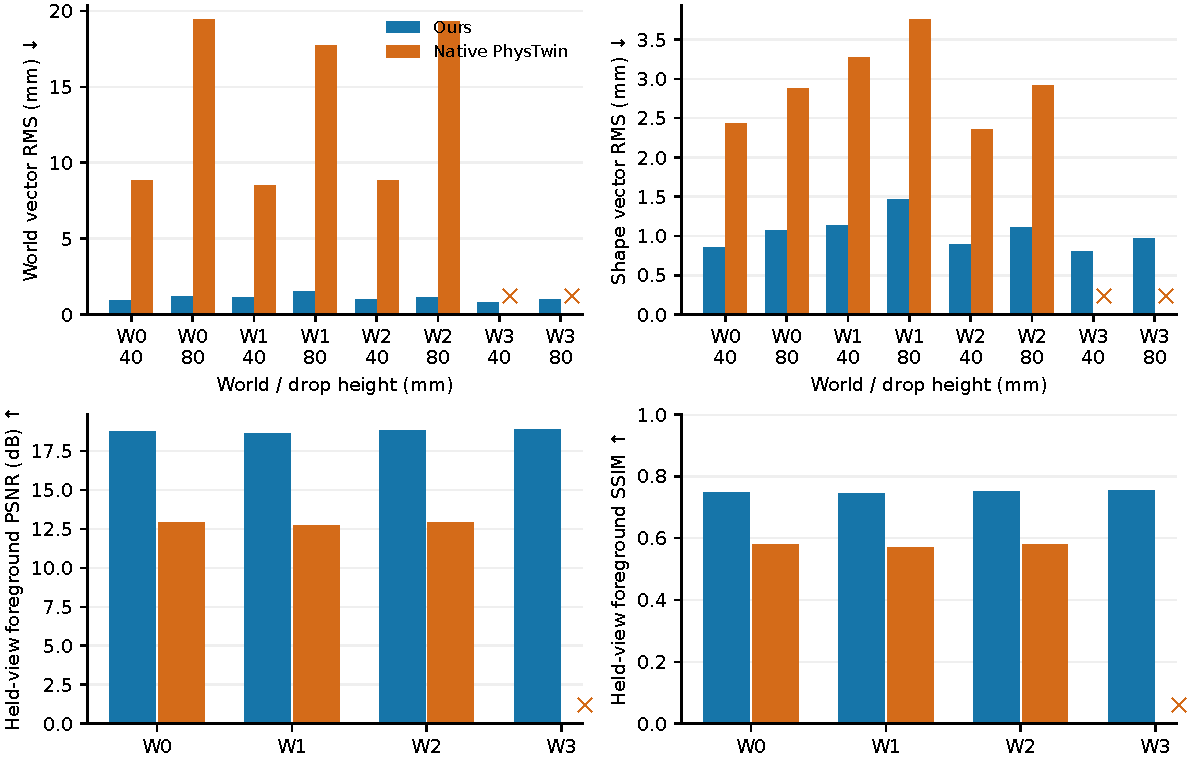
\includegraphics[width=.84\textwidth]{figures/dynamic_results.pdf}
\caption{\textbf{All declared dynamic cases.} Top: world and rigid-aligned shape errors for both forecast heights in each world. Bottom: held-view image metrics by world. Crosses mark unavailable native predictions in world 3; they are not zero-valued measurements. Shared appearance initialization makes the image comparison a test of predicted motion plus Gaussian transport.}
\label{fig:dynamics}
\end{figure*}

\subsection{Earlier drop-cohort appearance illustration}
Figure~\ref{fig:qualitative} illustrates the earlier four-world drop study; the six-family experiment below uses a separate held cohort.
\begin{figure*}[t]
\centering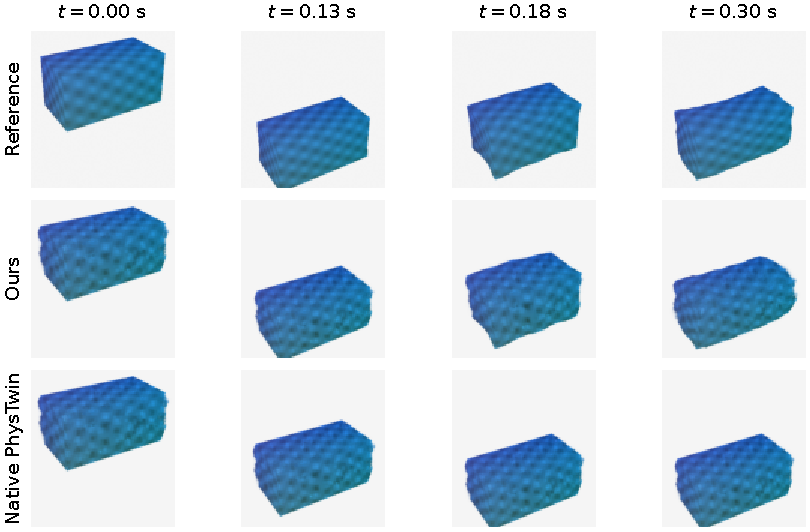
\includegraphics[width=.80\textwidth]{figures/qualitative.pdf}
\caption{\textbf{Earlier four-world drop cohort: reference versus predicted appearance.} First declared world, 80\,mm forecast, first held camera. The same crop is computed across all methods and all 31 frames; RGB values are unchanged. Columns show 0, 0.13, 0.18 and 0.30\,s. This selection is a fixed case illustration, not an aggregate result. Supplementary videos include all eight forecasts, including the unavailable native case.}
\label{fig:qualitative}
\end{figure*}

\section{Six-family coupled-scene benchmark}
\label{sec:complex-scenes-supp}
\subsection{Coupled-scene prediction protocol}
\label{sec:coupled-protocol}
We separate the material of an object from the interaction applied to it.
A world $w$ specifies fixed object geometry, density, and a hidden material
field $m_w$. An interaction $a$ specifies the initial state, prescribed fixture
positions and release schedule, gravity, and collision geometry. For each
world, a short calibration interaction provides point observations
$\mathcal D_w=\{(t_i,X_j,x_{ij})\}$ up to a fixed cutoff. A method fits its
material representation to this prefix, seals the fitted parameters, and
predicts two different interactions without refitting. The same hidden
material is retained across calibration and both queries.

The protocol contains six scene families: moving and released compliant
clamps; pushing around a curved obstacle; gravity drops into a curved
container, including an obstacle; a translating finite-mass rigid striker;
two deformable objects in collision or stacking; and spatially heterogeneous
material. Query changes include fixture location, displacement amplitude,
impact velocity, drop height and orientation, and contact configuration.
The frozen census is four independently sampled material worlds per
family and two queries per world. Object shape and density are fixed in
this study; transfer is across material and interaction, rather than unseen
object geometry.
The protocol, implementation inventory, model checkpoints, and development
decision were fixed before generating the held worlds. Young's modulus is
sampled log-uniformly from $8$ to $18$\,kPa and Poisson's ratio uniformly
from $0.25$ to $0.40$. Two-body scenes use independent material draws.
Heterogeneous worlds additionally sample a log-contrast corresponding to
factors between two and three and a transition coordinate between $0.35$
and $0.65$. These draws remain fixed across each world's three interactions.

All methods receive the same calibration tracks, rest geometry, density,
and public boundary parameters. Tracks cover a fixed two-face material-point
subset and are sampled every $2$\,ms. This controlled track-input study does
not measure image tracking errors or camera-dependent occlusion. Materials
are unknown, while fixture compliance and collision geometry are known.
Consequently, this experiment evaluates prediction conditional on supplied
boundaries; it is not an evaluation of unknown-boundary recovery.

\subsection{Shared neural material with spatial descriptors}
The pretrained energy decoder is kept fixed. We infer a small spatial
material descriptor from the calibration prefix. For material coordinate
$X\in[0,1]^3$, the scale field is
\begin{equation}
 s_b(X)=s_0+\mathbf{1}_{b=2}\Delta s+
 c\tanh\!\left(8(X_1-r)\right),
\end{equation}
where $b$ indexes the deformable body. The same field parameterization is
available in every family; the heterogeneous-scene label does not switch
on a privileged material model. A second body receives an additional scale
offset, while the spatial profile and compressibility parameter are shared.
The other two pretrained descriptor coordinates are fixed at their
values $(0,-1)$ in this experiment.

We extend the frozen decoder with an independent positive multiplier on
its volumetric contribution. Writing $W_\theta$ for the pretrained energy,
$J=\det F$, and $B_\theta(s)$ for its existing positive volumetric
coefficient, the extension is
\begin{equation}
 W_{\theta,\beta}(F,s)=W_\theta(F,s)
 +(e^\beta-1)B_\theta(s)(J-\log J-1).
\end{equation}
Thus $\beta=0$ recovers the previous model exactly. The descriptor parameters
are fitted by bounded derivative-free optimization of the observed
point-position loss. No network weights are updated on a held world.
Additional calibration stages, when selected in development, initialize
from the preceding sealed best fit to the identical observation prefix.
This changes the optimization budget without reading the future query.
The frozen schedule permits $64$ objective evaluations followed by up to
$128$ additional evaluations, initialized from the best calibration fit.
The analytic control receives the identical schedule. The best calibration
loss determines the parameters used for both queries; no query-specific
parameter selection is performed. Reaching an evaluation limit is reported
separately from optimizer convergence.

Predicted motion follows the coupled mechanics rollout with explicit
collision geometry and compliant fixtures. The current scene model includes
conservative penalty contact, separation, and translation of the rigid
sphere; it does not model general rotating rigid shapes, friction, or
continuous collision detection. These limits define the evaluated scene
capabilities rather than being hidden in an aggregate score.

\subsection{Adapted mechanics baselines}
We compare with PhysTwin~\cite{jiang2025phystwin},
Spring-Gaus~\cite{zhong2024springgaus}, and
UniPhy~\cite{mittal2025uniphy}, using pinned author implementations.
PhysTwin uses the author Warp spring-force kernel and native forecast
integration, with per-edge stiffness fitted to the common track prefix.
Spring-Gaus uses the author internal forces and integration, a scalar
stiffness initialization search, and subsequent per-edge fitting. Both use
known object masses and explicit common scene-boundary adapters. PhysTwin
uses fixed zero dashpot and drag damping in this adapter. These are
mechanics comparisons with disclosed interfaces, not reproductions of the
complete author image-reconstruction pipelines.
Both native spring adapters use $40$ Adam iterations with learning rate
$0.03$ and a four-hour fitting limit. Spring-Gaus first searches a scalar
stiffness initialization. Single-clamp development controls at $160$
iterations improved calibration but increased vector forecast error for
both adapters; these controls and their shape errors are retained alongside
the selected budgets. This observation does not establish that $40$
iterations is optimal for every scene. Actual successful iterations and
numerical failures are reported rather than assumed from requested budgets.

UniPhy uses the released pretrained constitutive networks and native MPM,
with a fitted material latent and explicit bowl/obstacle hooks. Its current
adapter supports the drop family only. Its native separating-velocity
projection differs from the conservative penalty contact of the reference
and the other adapters; its results therefore measure this adapted
system's capability, not a matched-contact-law material-inference error.
Any adjoint adaptation and its derivative checks are reported separately.
Unsupported configurations are retained as unsupported, rather than being
counted as failures or wins. An analytic Neo-Hookean control uses the same
spatial fitting parameterization but has the advantage of knowing the
reference constitutive family.
UniPhy uses eight fixed-seed latent-centroid initializations followed by
eight AdamW iterations at learning rate $3\times10^{-5}$. Its derivative
qualification remains coordinate-sensitive, which limits attribution of
any adapted-system failure to the original method.

\subsection{Physical and visual evaluation}
We report full-query point-position RMS and per-object rigid-aligned shape
RMS separately. Additional physical diagnostics include sampled contact
penetration and first-contact time, net nongravitational body impulse,
and signed tetrahedron-volume ratios on the same material grid for all
methods. The impulse is computed from saved velocity and known mass after
subtracting gravity; it does not resolve individual contact forces.
Sampled orientation and gap checks are diagnostics, not proofs of global
injectivity or continuous nonintersection.

For a controlled image comparison, every method and the reference use the
same frozen Gaussian appearance, the same motion-transport map, and fixed
withheld cameras. We report PSNR, SSIM, LPIPS, and silhouette IoU, averaging
noninitial query frames for the primary scores and retaining all-frame
values separately.
This separates motion-induced image error from independent appearance
optimization. The rendering is object-only and does not test environmental
occlusion or native end-to-end reconstruction quality. Image agreement and
physical agreement are evaluated separately; neither is inferred from the
other.

Numerical reference uncertainty is assessed through spatial refinement,
with dense sampled orientation checks. A completed reference trajectory is
not automatically treated as spatially converged. Fitting, rollout,
reference and infrastructure failures remain separately visible in the
complete planned census. We average the two queries within each world,
then compute paired method differences and bootstrap intervals by resampling
worlds, not frames. Error comparisons conditional on successful paired
worlds are accompanied by their completion and coverage counts.
References use Q2 meshes with $(4n,n,n)$ cells, $n=4$, Lobatto-4 quadrature,
and a $25$\,$\mu$s time step. Both queries of the preselected first world
in every family are repeated at $n=6$. These twelve comparisons quantify
resolution sensitivity on those worlds; they are not rigorous error bounds
or a population-wide convergence certificate. Our material model and the
analytic control use $n=1$ with $50$\,$\mu$s steps. Native spring adapters
use $25$\,$\mu$s steps and UniPhy uses $50$\,$\mu$s steps.

\subsection{Held physical prediction results}
\label{sec:coupled-physical-results}
Ours, the analytic control, Spring-Gaus and PhysTwin each complete all
48 held queries. Table~\ref{tab:coupled-physical} summarizes full-query
motion errors, including the shared initial frame, and rigid-aligned shape
errors. The paired mean motion-error difference across 24 independent
worlds is $-8.83$\,mm against PhysTwin (world-bootstrap 95\% interval
$[-12.18,-5.83]$) and $-9.30$\,mm against Spring-Gaus
($[-12.40,-6.50]$). Our difference from the analytic control is
$+0.13$\,mm ($[-0.01,0.27]$); this does not establish an advantage over
the matched analytic family. The analytic control knows the reference
constitutive family but fits its unknown material parameters from the same
observed prefix.

\begin{table}[t]
\centering\small
\caption{Six-family held physical prediction. Motion and rigid-aligned
shape RMS are in mm. Folds counts queries with any nonpositive sampled
material-grid tetrahedron volume; this is a common diagnostic, not a
continuous-injectivity certificate. All rows complete 48/48 queries.}
\label{tab:coupled-physical}
\begin{tabular}{lrrr}
\toprule Method & Motion & Shape & Folds \\
\midrule
Ours & 1.97 & 1.25 & 0 \\
Analytic control & 1.84 & 1.16 & 0 \\
PhysTwin adaptation & 10.80 & 5.94 & 33 \\
Spring-Gaus adaptation & 11.27 & 6.00 & 37 \\
\bottomrule
\end{tabular}
\end{table}

Our mean motion error is lower than both native adaptations in each of
the six families. Against the analytic control, our descriptive mean is
lower for clamps/release, curved pushing, two-body interaction and
heterogeneous material, and higher for drops and rigid impacts.
These per-family results have four independent worlds each and should not
be interpreted as universal rankings.

The mean net nongravitational impulse error is $0.0098$\,N\,s for ours,
$0.0086$ for the analytic control, $0.0500$ for PhysTwin and $0.0572$
for Spring-Gaus. This metric compares momentum changes after subtracting
gravity; it does not identify individual contact forces.
The common sampled contact diagnostic records 44 body--collider or
body--body event identities per fully covered method. Ours and the
analytic control have no missed or extra contacts. Spring-Gaus has two
extra contacts and PhysTwin four, all in the two-body family; neither
has a missed contact. Mean absolute errors in maximum sampled penetration
are $2.85$, $2.27$, $4.37$ and $4.14$\,mm for ours, analytic, PhysTwin
and Spring-Gaus, respectively. These gaps are sampled and use the declared
normalized implicit bowl geometry; they are not exact overlap distances.

UniPhy's single completed query has motion error $18.41$\,mm and shape
error $15.69$\,mm. Seven supported queries fail numerically and 40 are
unsupported; no complete paired world exists for a comparative claim.
Eleven of twelve prospective $n=4$ versus $n=6$ reference comparisons complete.
The refined stacking query reaches its declared time limit; its unfinished
trajectory is not scored. Noninitial motion differences range from
$0.027$ to $0.931$\,mm, with the largest values in container drops.
These are resolution and contact-sampling sensitivities, not error bounds.
A post-hoc audit of unchanged predictions against the refined references
retains five fully paired worlds: mean motion-error differences for ours
minus PhysTwin and Spring-Gaus are $-7.20$ and $-7.87$\,mm, respectively
(compared with $-7.30$ and $-7.95$\,mm against the primary references on
the same subset). The analytic-control difference is $+0.20$\,mm.
This subset audit does not establish population-wide convergence. All primary query reference trajectories pass their declared
sampled Jacobian guard, with minimum dense sampled determinant $0.272$;
this does not establish spatial convergence.

\subsection{Held common-appearance results}
\label{sec:coupled-appearance-results}
Table~\ref{tab:coupled-appearance} reports all 48 queries for each fully covered method. All methods transport the same Gaussian appearance using the same rendering pipeline; this isolates image differences induced by predicted motion and is not a comparison of native end-to-end reconstruction systems.
\begin{table}[t]
\centering\small
\caption{Six-family held common-appearance evaluation. Foreground-union PSNR and SSIM and image LPIPS use noninitial frames. Means average the same 48 queries per row. Higher PSNR/SSIM and lower LPIPS are better.}
\label{tab:coupled-appearance}
\begin{tabular}{lrrr}
\toprule Method & PSNR & SSIM & LPIPS \\
\midrule
Ours & 35.61 & 0.877 & 0.0101 \\
Analytic control & 36.02 & 0.887 & 0.0093 \\
PhysTwin adaptation & 25.68 & 0.731 & 0.0404 \\
Spring-Gaus adaptation & 25.88 & 0.721 & 0.0425 \\
\bottomrule
\end{tabular}
\end{table}
Across 24 independent worlds, the paired foreground PSNR difference (ours minus baseline) is $+9.93$\,dB against PhysTwin (world-bootstrap 95\% interval $[8.24,11.76]$) and $+9.73$\,dB against Spring-Gaus ($[7.93,11.67]$). The analytic control is slightly better: our difference is $-0.41$\,dB ($[-0.77,-0.08]$). LPIPS differences favor ours over the two native adaptations, while favoring the analytic control over ours. These comparisons are specific to the declared adapters, observation prefixes and fitting budgets.

UniPhy completes one of eight supported drop queries; seven fail with a native CFL error. The other 40 slots are unsupported by this adapter. Because no UniPhy world completes both queries, no paired-world image comparison is reported. Its one completed query has foreground PSNR $12.24$\,dB; this isolated descriptive value is not comparable to the 48-query averages above.

Physical-error evaluation and the two remaining spatial-reference refinement runs are still in progress at this draft stage. Image fidelity alone does not establish mechanical accuracy.

\begin{table}[t]
\centering\scriptsize
\caption{Foreground PSNR by scene family (dB; eight queries each). Averages describe the frozen held cohort, not population guarantees.}
\label{tab:coupled-appearance-family}
\begin{tabular}{lrrrr}
\toprule Family & Ours & Analytic & Spring & PhysTwin \\
\midrule
Clamps/release & 28.78 & 28.96 & 19.91 & 20.06 \\
Curved pushing & 30.63 & 30.20 & 24.21 & 21.86 \\
Container drop & 45.37 & 45.83 & 27.78 & 27.82 \\
Rigid impact & 40.70 & 42.73 & 36.94 & 35.72 \\
Two soft bodies & 40.93 & 41.16 & 27.16 & 27.50 \\
Heterogeneous & 27.26 & 27.23 & 19.30 & 21.14 \\
\bottomrule
\end{tabular}
\end{table}

\subsection{Held comparison media}
The six-family media set contains twelve clips: the first predefined world
(world00) in every family, with both held interactions. This selection does
not depend on prediction errors. Each clip shows six panels: the simulation
reference, ours, the analytic control, Spring-Gaus, PhysTwin and UniPhy.
Unsupported and failed slots are labeled explicitly. Complete predictions
use synchronized saved physical times, the same orbiting camera and common
axis limits; deformation is not amplified. Playback is 24 frames per second
for states sampled every 2\,ms, corresponding to approximately $20.8\times$
slow motion. These checkerboard surface visualizations expose geometry and
interaction differences; they are separate from the common-Gaussian image
evaluation in Tables~\ref{tab:coupled-appearance}
and~\ref{tab:coupled-appearance-family}.
The local media filenames follow
\texttt{held-\{family\}-world00-query\{0,1\}.mp4}.
The accompanying audit records source trajectory hashes, movie hashes,
frame counts and successful full-stream decoding for all twelve clips.


\clearpage
\onecolumn
\section{Spatial error maps across all six scene families}
\begin{figure}[ht]
\centering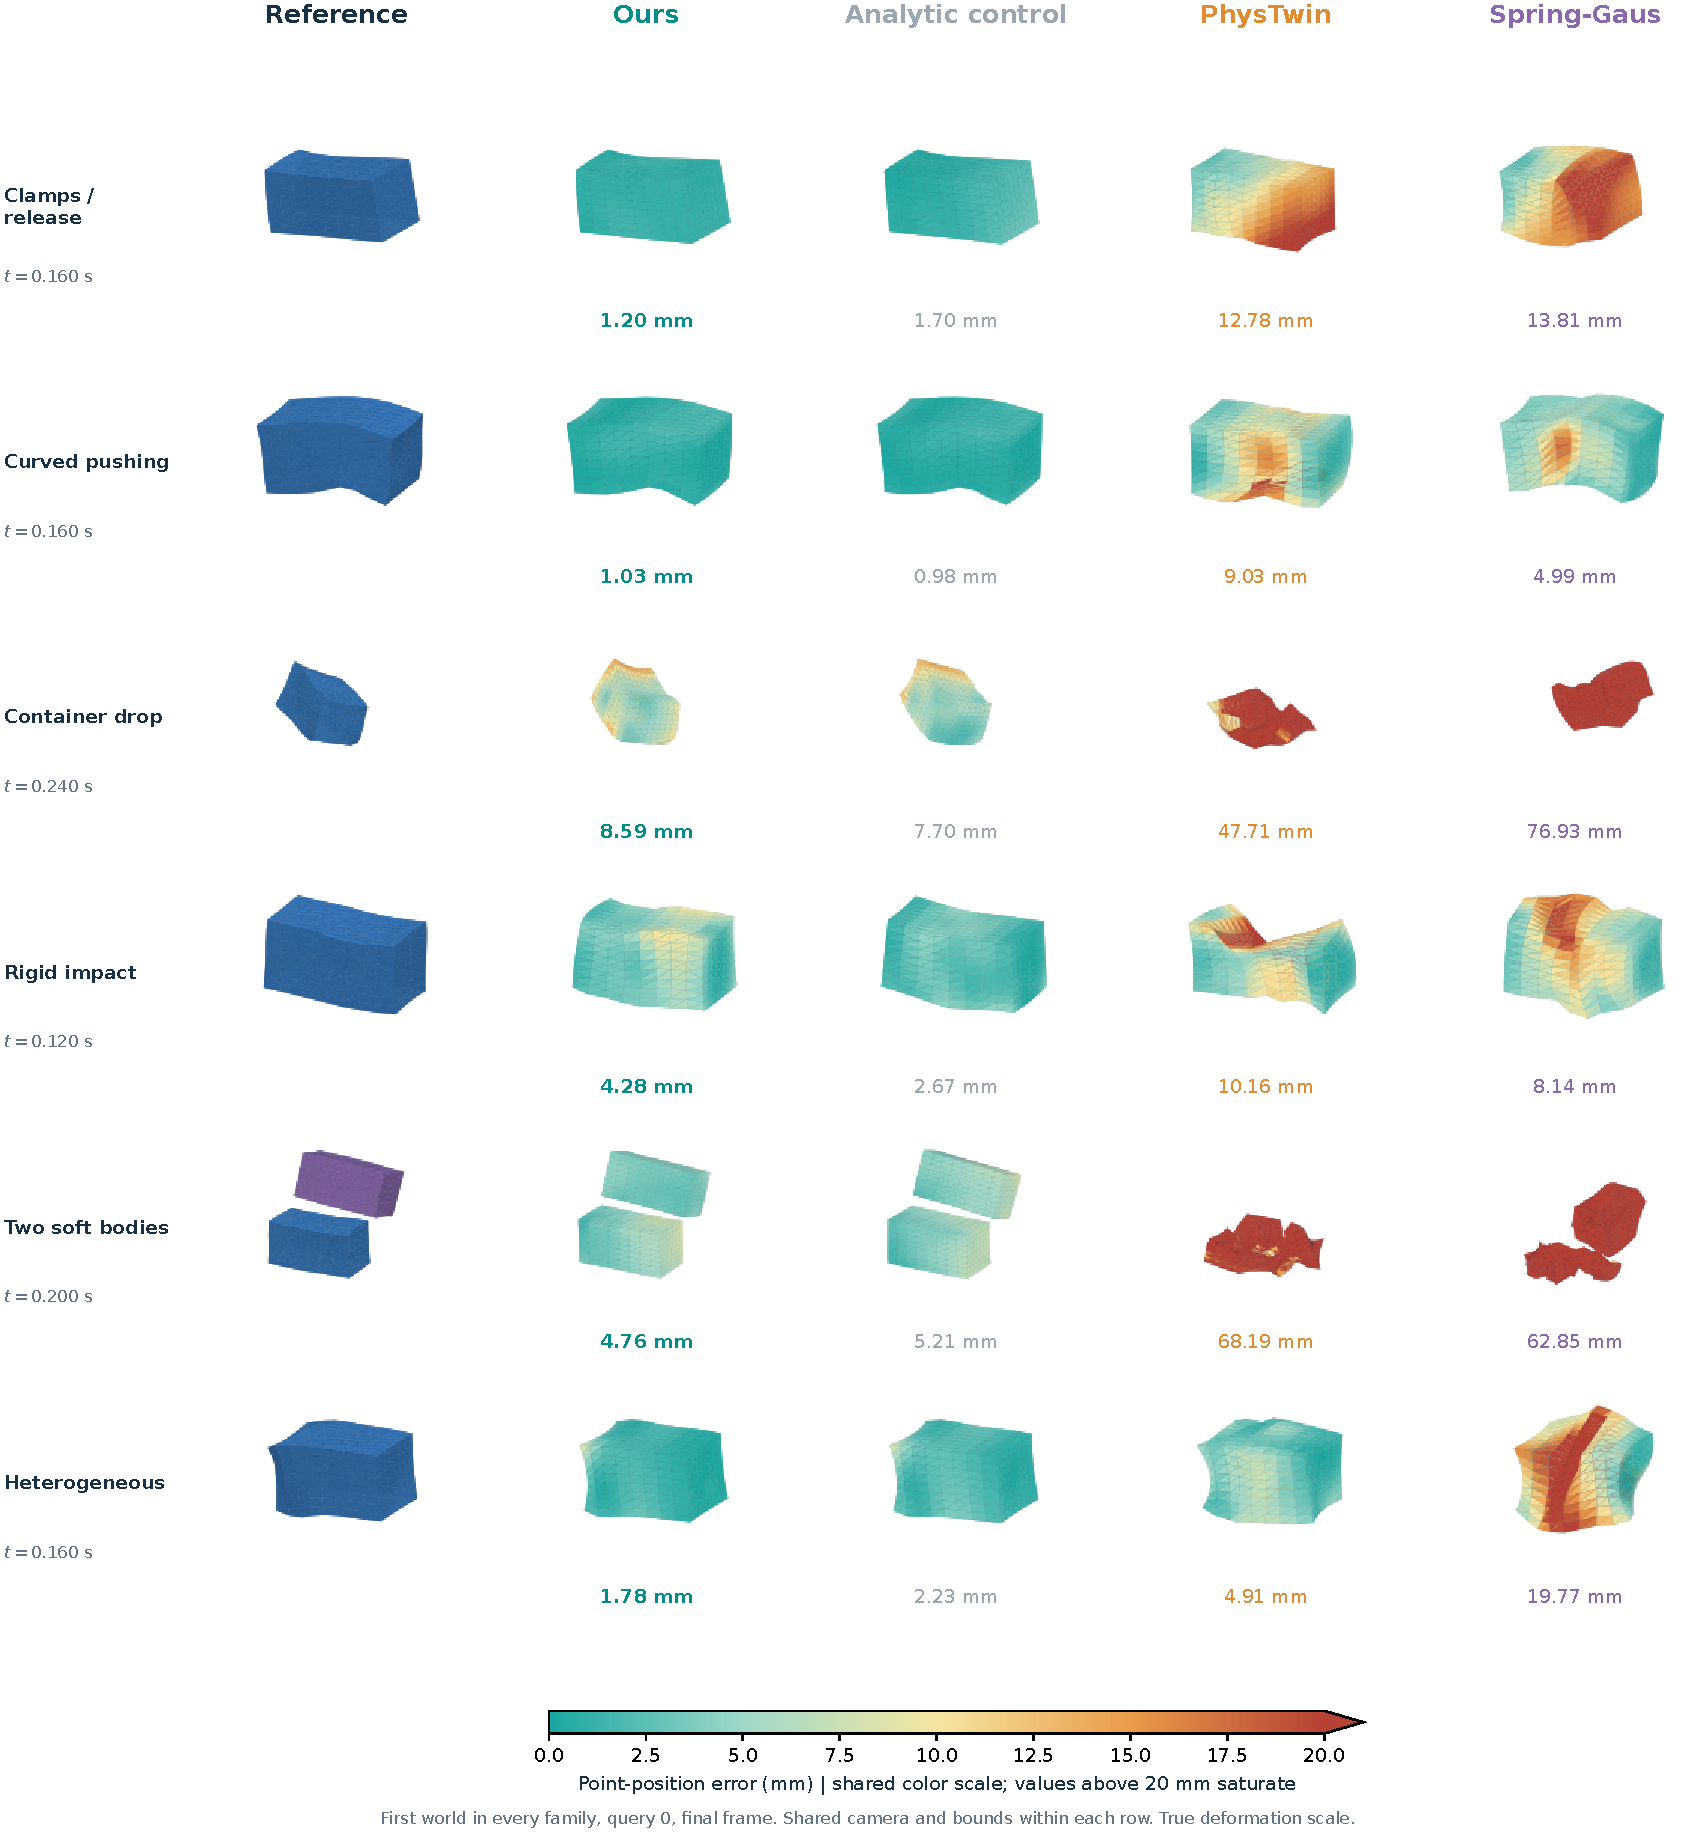
\includegraphics[width=.96\textwidth,height=.74\textheight,keepaspectratio]{figures/held_error_plate.pdf}
\caption{\textbf{Where the predictions differ from the reference.} Every family uses its first predefined world, query 0 and final frame, without outcome-based selection. The numbers are point-vector RMS for that frame, not full-trajectory averages. All prediction surfaces use one 0--20\,mm point-error scale; triangle colors average vertex errors and larger values saturate. Camera and spatial bounds are shared within each row; deformation is not amplified. Reference surfaces use a solid body color. This geometry diagnostic is separate from Gaussian image-quality evaluation. UniPhy is unsupported in five families and fails on this selected drop query; it has no completed surface to plot here.}
\label{fig:held-error-map}
\end{figure}
\clearpage
\twocolumn
{\small\bibliographystyle{ieeenat_fullname}\bibliography{references}}
\end{document}
